% !TeX root = ../main.tex
\subsection{\textit{ChromHMM} results} \label{chap: ChromHMM results} %#TODO change title

In total, 4 states were considered to be present. Two functions in particular were used: BinarizeBam and LearnModel. The data shown in \ref{methods: data used} were aligned to \textit{hg38} reference genome
\cite{HomoSapiensGenome}
. Results are shown in image \ref{fig:ChromHMM results}; by taking a look to its subfigures, the following considerations could be done:

\begin{enumerate}
  \item Clear absence or presence of ATAC and CTCF signals could be detected in figure \ref{fig:State emission parameters}. for this reason, the following states are defined:
  \begin{itemize}
    \item \textbf{State 1}: State without the presence of ATAC and CTCF signal
    \item \textbf{State 2}: State with ATAC but not CTCF peaks
    \item \textbf{State 3}: State with the presence of both ATAC and CTCF signal
    \item \textbf{State 4}: State with CTCF but not ATAC peaks
  \end{itemize}
  \item The states 1 and 2 in particular tend to perform transitions towards themselves instead of different states (figure \ref{fig:State transition parameters})
  \item State 2 (with ATAC) and 3 (with ATAC and CTCF) tend to localize in CpG islands, exons and Transcriptional Starting Sites (figures \ref{fig:State enrichment in genome}, \ref{fig:TSS state population}, \ref{fig:TES state population})
\end{enumerate}

\begin{figure}[H]
    \centering
    \begin{subfigure}[t]{0.06\textwidth}
      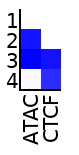
\includegraphics[width=\linewidth]{/home/maurizio/Documents/GitHub/Multiscale-Potestio/proj_multiscale/images/StateEmission_IMR90.png}
      \caption{State emission parameters}
      \label{fig:State emission parameters}
  \end{subfigure}
  \begin{subfigure}[t]{0.11\textwidth}
      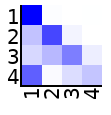
\includegraphics[width=\linewidth]{/home/maurizio/Documents/GitHub/Multiscale-Potestio/proj_multiscale/images/StateTransition_IMR90.png}
      \caption{State transition parameters}
      \label{fig:State transition parameters}
  \end{subfigure}
  \begin{subfigure}[t]{0.15\textwidth}
      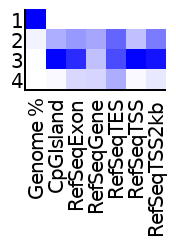
\includegraphics[width=\linewidth]{/home/maurizio/Documents/GitHub/Multiscale-Potestio/proj_multiscale/images/EnrichmentInRegions_IMR90.png}
      \caption{State enrichment in genome}
      \label{fig:State enrichment in genome}
  \end{subfigure}
    \hspace{0.6\textwidth}
    \begin{subfigure}{0.39\textwidth}
      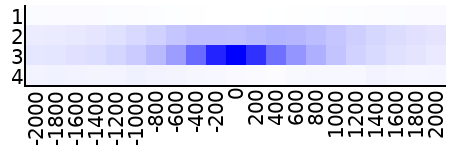
\includegraphics[width=\linewidth]{/home/maurizio/Documents/GitHub/Multiscale-Potestio/proj_multiscale/images/TSSpopulation_IMR90.png}
      \caption{TSS state population}
      \label{fig:TSS state population}
    \end{subfigure}
    \begin{subfigure}{0.39\textwidth}
      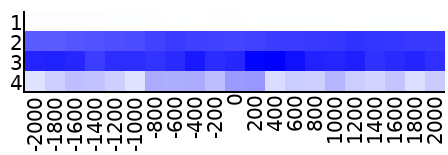
\includegraphics[width=\linewidth]{/home/maurizio/Documents/GitHub/Multiscale-Potestio/proj_multiscale/images/TESpopulation_IMR90.png}
      \caption{TES state population}
      \label{fig:TES state population}
    \end{subfigure}
  
    \caption{Results from ChromHMM for the IMR90 replicates}
    \label{fig:ChromHMM results}
\end{figure}


The proportions represented in image \ref{fig: proportions in bins} were obtained. In general, the proportions calculated taking into consideration the segments are much lower with respect to those calculated with the bins. The reason is that the first state is in general much more present than the other three. The ratios are larger with 5 kbp bins as in fact whenever there are a few occurrences of the rarely present states, those are assigned with a great probability and convert a great number of segments which are not anymore assigned to state 1.

\begin{figure}[H]
  \centering
  \begin{subfigure}[t]{0.45\textwidth}
    \includegraphics[width=\linewidth]{/home/maurizio/Documents/GitHub/3DCS/Maurizio/steps/2-state_5kb/images/200_segm_IMR90.png}
    \caption{Proportions of states in 200 bps segments. The segments were directly found by \textit{ChromHMM}. Each dot represents the proportion relative to a chromosome.}
    \label{fig: proportions in segments}
  \end{subfigure}
  \begin{subfigure}[t]{0.45\textwidth}
      \includegraphics[width=\linewidth]{/home/maurizio/Documents/GitHub/3DCS/Maurizio/steps/2-state_5kb/images/5000_bins_IMR90.png}
      \caption{Proportion of states in 5000 bps long bins. Each dot represents the proportion relative to a chromosome.}
      \label{fig: proportions in bins}
  \end{subfigure}
  \caption{Proportions found in 200 bp segments and in 5000 bins.}
  \label{fig: proportions bins and steps}
\end{figure}


The following image \ref{fig: ANPEP igv} was created by using IGV, a visualization tool
\cite{robinsonIgvJsEmbeddable2020a,robinsonIntroductionIntegrativeGenomics}
. After a visual inspection of the results, it was decided to trust the assignment performed. However, some defects become evident while viewing the results: whenever the \textit{ChromHMM} signals the presence of the $4^{\text{th}}$ state, the relative bin is assigned to it. What happens is that, when the fourth state is found, if the $3^{\text{th}}$ (with both ATAC and CTCF) is not enoughly signaled, the information about the presence of ATAC peaks is lost. Problems about the precision of the state assignment process couldn't be easily solved and are a direct consequence of the coarse-graining process.
%#TODO maybe you find a solution

\begin{figure}[H]
  \centering
  \includegraphics[width=\linewidth]{/home/maurizio/Documents/GitHub/3DCS/Maurizio/steps/2-state_5kb/images/igv_ANPEP.png}
  \caption{IGV snapshot of a portion of the ANPEP region analyzed. The first track reports the alignment results obtained from the ATAC data, the second the CTCF data}
  \label{fig: ANPEP igv}
\end{figure}
